\subsection{Sous-mission B2} 

	\begin{vwcol}[widths={0.8,0.2}, rule=0pt]
	\begin{minipage}{0.7\textwidth}
	\paragraph{Objectifs de la mission}

	L'objectif de cette mission était d'améliorer la visibilité de l'image afin de la donner à un autre service pour identifier la position d'une naine blanche située à 150 années lumière de la Terre.
	\end{minipage}
	\begin{minipage}{0.2\textwidth}
		\begin{flushright}
			\paragraph{Filtre utilisé}

			Normalisation
		\end{flushright}
	\end{minipage}
	\end{vwcol} 

	\begin{figure}[h]
	\centering
		\begin{multicols}{2}
		
\includegraphics[scale=0.525]{images/GD61.png}
		Avant
		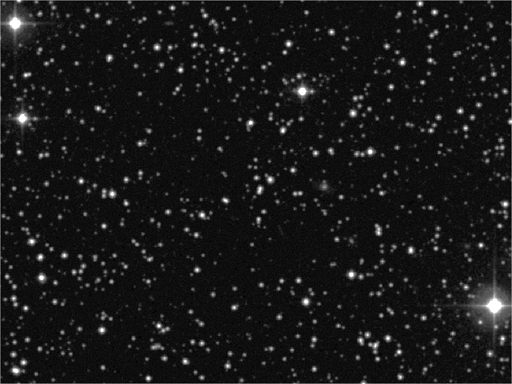
\includegraphics[scale=0.525]{images/GD61AFTER.png}
		Après
		\end{multicols}
	\end{figure}
	\vspace{-0.9cm}

		\paragraph{Procédé}	
			Pour cette mission une normalisation a été réalisée, faisant clairement apparaître les différentes planètes et étoiles.